\documentclass[12pt,a4]{article}
\usepackage{amsmath,amsfonts,amsthm,amssymb, mathtools,steinmetz, gensymb, siunitx}	% LOADS USEFUL MATH STUFF
\usepackage{xcolor,graphicx}
\usepackage[left=1.5cm, top=2cm, right=1.5cm, bottom=2cm ,a4paper]{geometry} 				% ADJUSTS PAGE
\usepackage{setspace}
\usepackage{caption}
\usepackage{tikz}
\usepackage{pgf,tikz,pgfplots,wrapfig}
\usepackage{mathrsfs}
\usepackage{fancyhdr}
\usepackage{float}
\usepackage{array}
\usepackage{unicode-math}
\usepackage{booktabs,multirow}
\setmathfont{Libertinus Math}

\usetikzlibrary{decorations.text}
\pgfplotsset{compat=1.7}

\usetikzlibrary{decorations.pathreplacing,decorations.markings}
\usepgfplotslibrary{fillbetween}

\usepackage{hyperref}
\usepackage[style=ieee, maxbibnames=6, minnames=1,maxnames = 1]{biblatex}
\addbibresource{references.bib}


\AtBeginDocument{\hypersetup{pdfborder={0 0 0}}}

\title{

\includegraphics[scale = 0.5]{download.jpg}~ 
\\[1cm]
\textsc{Real Time Detection and Tracking of People in Crowds}
}
\author{\textsc{J L Gouws}
\\Supervisor: \textsc{Mr. J Connan}
\\ \emph{Computer Science Department, Rhodes University}}
\date{\today
\\[1cm]}



\usepackage{graphicx}
\usepackage{array}




\begin{document}
\fontencoding{T1}
\fontfamily{ppl}\selectfont
\thispagestyle{empty}

\maketitle

%In some sections you have to make a best guess (hypothesis), since you haven't done your MSc yet. 
\begin{abstract}
  Tracking of objects in videos streams is a powerfull tool in the field of computer vision.
  It is, however, a relatively unexplored field when compared to other areas of computer vision.
  That being said, there have been impressive developments in the field in recent years.
  I propose to use methods of machine learning and image processing to further explore object tracking and detection.
  The specific focus of my research will be the detection and tracking of people in crowds.
  Another concern of the research is performance of the implemented system.
  A large amount of computation power is often needed to analyze videos of crowds, investigation into reducing the required computation power of this system will also be carried out.
\end{abstract}

\newpage
\section{Introduction}
  This document is a literature review for the associated Honours project.
  This paper also serves to revise the proposal.
  Below is an amended introduction to the project.

  Consider a continuous video stream where a set of faces appears, and each face might appear at different times.
  The individual faces might move and change orientation in the video stream.
  Imagine that some subset of these faces is of interest--the target faces.
  A set of pictures of these faces must exist; these pictures may be unrelated to the video or frames within it.
  This research aims to develop a system that solves the problem of automatic identification and tracking of target faces in the video stream.

  The initial input given to the system is images that have uniquely labelled regions of interest or bounding boxes which define individual faces.
  The input images must contain at least one instance of each target face, but there is no maximum limit.
  This process constitutes the initialisation of operation, after which the system functions autonomously.

  Given an arbitrary video, the system searches for the presence of any target faces.
  The tracker proceeds to label detected target faces with the label provided in the initialisation of the system.
  Once a target face is labelled, the tracker follows its motion, and all other targets appearing in the current frame.
  This process constitutes the running phase of the system, where the system identifies and tracks faces in the supplied video stream.

  While the system is running, it determines information about the target faces.
  It can, hence, extract the number of times each target face appears, the amount of time for which each target appears and the trajectory of each face while it is apparent in the video.
  This process is the output stage, which concludes the system's operation.

  The system operates with minimal input data supplied in the initialisation stage.
  With this constraint, the system should use all the data it can access. 
  Thus, the system uses the video to learn more about each target face in the running phase.
  In this way, the system can identify and track faces with better accuracy as the video progresses.

  The next section of this document reviews the formal research statement.
  Following this, three sections introduce works that are related to this research.
  This section serves as the literature review of the project. 
  The literature review is followed by a section discussing the project's methodology.
  Finally, the conclusion summarises the literature review findings and details of the project.

\input{researchstatement}
\input{researchobjectives}
\section{Related Works}\label{sec:relatedWorks}
In 2011 \citeauthor{Kalal2011} invented the Tracking, Learning and Detection(TLD) framework for the longterm tracking of objects in a video stream.
Kalal's original implementation uses a median flow tracker, P-N learning, and a random forrest based detector \cite{KalalPHD}.
These three components give the respective tracking, learning and detection components of the system.

The learning compenent of TLD forms the backbone of the system governing the interaction between the detector and tracker.
The three components exchange information as shown in Figure~\ref{fig:tld}, this allows the tracker to improve it's performance as time progresses \cite{Kala2011}
The system requires online learning, learning as data becomes available, in order for the system to work. 
Kalal developed the P-N Learning paradigm \cite{PNLearning}, a semi-supervised bootstrapping model \cite{murphy2012machine}, tailored to the needs of TLD.

\begin{figure}{l}{0.55\textwidth}
   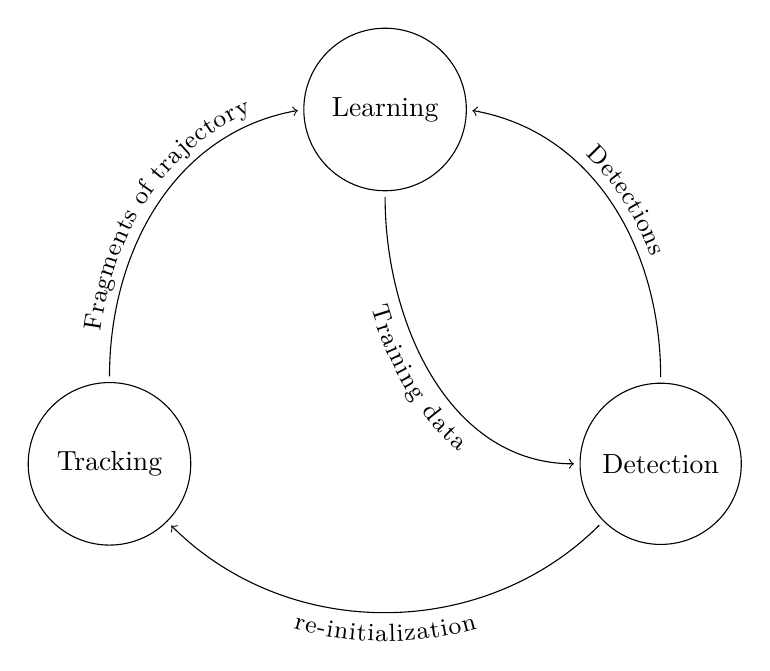
\begin{tikzpicture}[approach/.style={draw,very thick, fill=white, text width=5em,
         text centered, minimum height=2em,rounded corners=3ex, scale=0.1, everynode/.style={scale=0.1}},
         idea/.style={draw=black, circle,text width=5em,
            text centered, minimum height=2.5em},
         connections/.style={->,draw=black,shorten <=2pt,shorten >=2pt},
         reverseConnections/.style={<-,draw=black,shorten <=2pt,shorten >=2pt},
      ]

      \node[draw] at (0,0) (tracking) [idea]  {Tracking};
      \node[draw] at (3.5,4.5) (learning) [idea]  {Learning};
      \draw[connections, postaction={decorate, decoration={raise=1ex, text along path, text align=center, text={|\small|Fragments of trajectory}}}] (tracking.north)to[out=90,in=190] (learning.west) ;
      \node[draw] at (7,0) (detection) [idea]  {Detection};
      \draw[connections, postaction={decorate, decoration={raise=-2.5ex, text along path, text align=center, text={|\small|Training data}}}] (learning.south) to[out=270,in=180] (detection.west) ;
      \draw[reverseConnections, postaction={decorate, decoration={raise=1ex, text along path, text align=center, text={|\small|Detections}}}] (learning.east) to[out=350,in=90] (detection.north) ;
      \draw[reverseConnections, postaction={decorate, decoration={raise=-2.5ex, text along path, text align=center, text={|\small|re-initialization}}}] (tracking.south east) to[out=-45,in=225] (detection.south west) ;
   \end{tikzpicture}
   \caption{The interaction between tracking, learning and detection in TLD. Figure from \cite{Kalal2011}}
   \label{fig:tld}
\end{figure}

\citeauthor{Enriques2014} \cite{Enriques2014} propose Kernelized Correlation Filters(KCF) and the novel Dual Correlaion filter(DCF).
Both KCF and DCF use circulant matrices and the kernel Trick.

applied on Histogram of Oriented Gradient features.

The system developed by \citeauthor{Enriques2014} does not encorporate a failure recovery mechanism--section 8 of \cite{Enriques2014}.
This is in contrast to the TLD system which provides a failure recovery mechanism in the detection component \cite{Kalal2011}.
KCFs also require a stage that will start them tracking.
KCFs have great potential to be used as the tracking stage for a TLD tracker.

Kalal uses Random Forest for detection in his implementation of TLD.
A more modern approach would be to use Extreme Gradient Boosting(XGB) for the detector.
XGB generally offers similar if not better classification performance than Random Forest and requires significantly less time to train \cite{comparativeXGB}.

There has also been investigation into the use of Convolutional Neural Networks in tracking \cite{CNNTracking}.
This offers high performance tracking of generic objects.
It will be investigated for extension to tracking and detecting people in crowds.
It will not be a main point of research unless it turns out to be fruitful--seeing as CNNs tend to require large amounts of training time, data, and memory space.

There has also been some quite old research that involves localizing multiple targets.
The research of Taylor and Drummond \cite{taylorDrummondTracking} offer this at high FPS even on low powered devices.

Currently there are vary many trackers availble all with varying degrees of performance.
These have been benchmarked in \cite{VOT2017} and \cite{VOT2020}.
This is a good reference, and will be explored further, but not all trackers can satisfy the requirements of this project. 

There has also been relevant work done on correlation tracking by \cite{Ma2015Correlation}.
Ma. et al investigated the problem of long term tracking where the target undergoes abrupt motion, heavy occlusions and disapearing from view.
There work will probably integrate well with Kernelized Correlation filters, and it has very practical advantages.
It is not the forefront of this research to handle occlusions, but it is a possible extension.

The P-N learning system is not completely unrelated to Reinforcement Learning Techniques.
There have been promising recent results in online reiforcement learning \cite{onlineRL}.
The work of \cite{onlineRL} allows for variable data budgets, which should integrate well with a constant flux of input from a video stream.
TLD may not be compatible with the methods proposed in \cite{onlineRL}, but the feaibility of the ideas will be explored in the paper.

\subsection{Approach to Research}
  The first phase of this research will consist of an in-depth reading of literature and further literature reviews.
  The literature reviews will start by reviewing Kalal's work on TLD.
  After a thorough review of Kalal's work, the research requires a review of works describing trackers other than TLD.
  Following this, there will be a further review of the literature discussing the online training of classifiers.
  Implementing the system requires data for testing--a brief phase of data acquisition from public sources will provide data for developmental and testing purposes.
  This material accumulation should suffice for the literature review and data collection.

  The second stage of this research will relate to the practicalities of the system's implementation.
  The language of the system's development is C++; The implementation requires a proficient understanding of the C++ language.
  Implementation requires an Investigation of the OpenCV C++ library and other available utilities at this point of the approach.

  The third phase consists of a functional reimplementation of the original TLD.
  Testing of this base system is required at this point so that problems do not occur in later stages of the full system implementation.
  Following the satisfactory performance of the TLD reimplementation, the next stage of research will commence.

  At this point, the base TLD system requires further improvement.
  The improvement will focus on the tracking and detection components of the system. 
  These improvements involve keeping the base model and improving the individual tracker parts or restructuring the model to improve performance.
  This phase will constitute the fourth stage of the research.

  Following this, the research investigates extending the system to track multiple objects simultaneously.
  There are naive ways to implement many object tracking systems, for example, creating many different single-target trackers to detect and track each object. 
  This stage requires significant planning, research and reviewing of the current implementation to achieve good model performance and efficiency.
  This stage completes the implementation of the system.

  The final stage of this research involves three things.
  First, the system requires a full review to find the strengths and faults of the design.
  If improvements to the implementation are required and time permits, development returns to stage four.
  Second, the system does test runs on videos obtained from the initial phase of the research for performance evaluation.
  Third, a thesis describes the implementation and specifications of the system.
  This step completes the research project.

\subsection{Timeline}
The timeline for this project has been revised since the Proposal version.
Most of the implementation deadlines now fall in the June and July Holiday, this is on account of exams and busy term times.
\begin{center}
  \begin{tabular}{l l}
    \toprule
      Time & Deliverable\\
    \midrule
      30 March 2022     & Seminar 1: Presentation of project\\
      11 April 2022     & Draft proposal\\
      19 April 2022     & Final proposal\\
      6 May 2022        & Literature review\\
      20 May 2022       & Obtaining suitable public videos\\
      25 June 2022      & Functional re-implementation of TLD\\
      28 June 2022      & Using KCF as Tracking stage of tracker\\
      30 June 2022      & Implementing DCF and comparing to KCF\\
      6 July 2022       & Reviewing VOT for better trackers\\
      11 July 2022      & Investingating random fern detectors\\
      11-13 July 2022   & Seminar 2: Progress Presentation\\
      25 July 2022      & Final decision on Tracking and Detection stages.\\
      12 August 2022    & Extension of system to multiple targets\\
      19 August 2022    & Progress Report\\
      26 August 2022    & Test and make small improvements the system\\
      3 October 2022    & First Draft of thesis\\
      10 Octorber 2022  & Completion of implementation\\
      14 October 2022   & Short ACM-style paper\\
      17-19 October 2022& Seminar 3: Final Oral presentation\\
      28 October 2022   & Final project submission\\
    \bottomrule
  \end{tabular}
\end{center}

\section{Limitations}
  It is difficult to accurately identify people from the rear.
  In this case it might be good to try and prevent the system from learning the appearance of the back of a person's head.
  A solution to this problem is also developing a system that can be distributed so as to be able to track people from a surrounded view.

  It is possible to track semi-ocluded targets, but detecting them is difficult.
  This will cause problems for the initialization and re-initialization of the tracker.
  It might be possible to impute some facial features before inputing the stream into the detection system.
  If a face is fully ocluded, however, there is not much that the system will be able to do, but a human will not be able to do very much.

  The system will require relatively good resolution cameras in order to identify people accurately from a long distance.
  In most situations involving crowds, a camera capturing a video stream will need to be placed a significant distance from the targets.
  Hence, the best we can do in software is try to use image processing techniques to artificially enlarge the target, or work on detectors that can work on minimal resolution.

\section{Applications}
  This reaseach has multiple real world applications.
  One includes an automated class register that can be used in schools or for university lecture attendance.

  Another application on the larger scale is a security system for monitoring the motion of people.
  This application requires the system to be extended to a distributed system.
  This could enhance airport security for example, adding functionality to label suspected terrorists.

  The system also has potential to be used as an assistive technology for visually impaired people.
  If the system can be ported to a mobile device, it could help a visually impaired person identify people at a party or on a television program.
  This application assumes the system has had the appropriate offline training in it's initialization phase.

\section{Conclusion}
\subsection{Revised Project Conclusion}
This research uses the Tracking, Learning and Detection(TLD) framework to implement a system that can track and detect multiple faces simultaneously.
TLD is used in the research to develop a long-term tracker that can recognize human faces and follow the trajectory of the faces in a video stream.

The system that the research implements is tested on public data.
Testing is done by having the system extract information about faces that appear in a given video stream.
The information collected by the implemented system is the number and duration of appearances for each target face. 

The research is limited to the tracking of faces, and is not aimed at tracking general objects or other human features.
Owing to the time limitations of an honours project, this project has substantial dependence on research done by other people and available tools.



\printbibliography

\end{document}
